\section{Reordering}
Another method to decrease the memory, needed to solve the transport of
electron, consists in reordering the groups. When CEPXS creates the cross sections,
it puts the first all the cross sections for one particle and then he puts the
cross sections for the order particles.  The cross section matrix looks like
\begin{equation}
S = 
\begin{pmatrix}
A & B\\
C & D
\end{pmatrix}
\end{equation}
where $A$ and $B$ are lower triangular matrices which represents the
scattering for the 2 particles types. For each particles, only down scattering
is allowed because the cut-off energy forbids the thermalization of the
particles. The matrices $B$ and $C$ represent the creation of electrons by
photons, through photo-electric effect, and the creation of photons by
electrons, through bremsstrahlung. Now it is important to notice that a
particle can only creates a particle which has a energy lower than its own
energy. Moreover, CEPXS forces the maximum energy and the cut-off energy to
be the same for the 2 particles. So if, for example, for the photons
there are 2 groups and for the electrons there are 4 groups, the transfer between
the groups will look \hbox{like :}
\begin{figure}[H]
\begin{center}
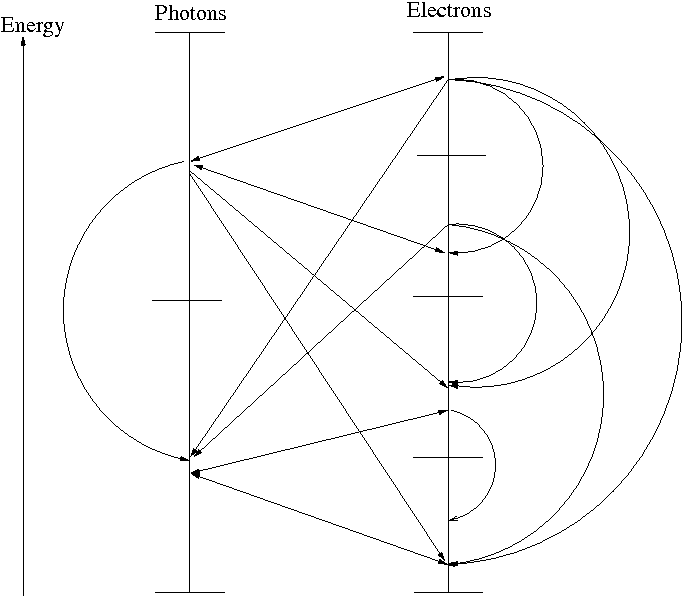
\includegraphics[height=7cm]{group.png}
\caption{Transfer between the different groups}
\end{center}
\end{figure}
and the pattern of scattering matrix looks like :
\begin{equation}
S =
\begin{pmatrix}
x & 0 & x & x & 0 & 0\\
x & x & x & x & x & x\\
x & 0 & x & 0 & 0 & 0\\
x & 0 & x & x & 0 & 0\\
x & x & x & x & x & 0\\
x & x & x & x & x & x\\
\end{pmatrix}
\end{equation}
We can see that that there is no upscattering to the first group of photons, the
first and the second group of electrons coming from the second group of photons,
the third or the fourth group of electrons. Thus, if we reorder the groups using the
following order : photon group 1, electron group 1, electron group 2, photon
group 2, electron group 3, electron group 4. The pattern of the scattering matrix
will looks like :
\begin{equation}
S =
\begin{pmatrix}
x & x & x & 0 & 0 & 0\\
x & x & 0 & 0 & 0 & 0\\
x & x & x & 0 & 0 & 0\\
x & x & x & x & x & x\\
x & x & x & x & x & 0\\
x & x & x & x & x & x\\
\end{pmatrix}
\end{equation}
Now, we see that we can solve our problem by solving 2 problems with only 3
groups each (we say that we have 2 group sets of 3 groups each). First we can solve 
the first 3 groups without taking care of the last 3 groups since there is no 
upscattering coming from these groups. Then, we can solve the last 3 groups, with 
the first 3 groups hidden in the source term. Thus, we can solve a problem with 6 
groups using the same memory that we would use for only 3 groups. To know how many 
groups from each particle we need to gather in each group set, we can use :
\begin{itemize}
\item The number of groups of photons is $n_p$, the number of groups of electrons 
is $n_e$ and the greatest common divisor between these 2 numbers is $gcd$
\item Number of groups of photons to put in a group set = $\frac{n_p}{gcd}$
\item Number of groups of electrons to put in a group set= $\frac{n_e}{gcd}$
\end{itemize}
Thus, instead of solving 1 problem of $n$ groups, we can solve $gcd$ problems
of $\frac{n}{gcd}$ groups.


